%%%%%%%%%%%%%%%%%%%%%%%%%%%%%%%%%%%%%%%%%%%%%%%%%%%%%%%%%%%%
%%                     Lösung Aufgabe 1                   %%
%%%%%%%%%%%%%%%%%%%%%%%%%%%%%%%%%%%%%%%%%%%%%%%%%%%%%%%%%%%%

\subsection{Impuls- und Sprungantwort 1} \label{aufg:1a}

Skizze der Impulsantwort $h_1[n] = (\frac{1}{2})^n ~u[n]$:

\begin{figure}[h]
    \centering
    \plotsequence{{1/0, 0.5/1, 0.25/2, 0.125/3, 0.0625/4}}{$h_1[n]$}
    \caption{Impulsantwort $h_1[n]$}
    \label{fig:h1}
\end{figure}

Sprungantwort:

$$
g_1[n] = (h_1*u)[n] = \sum_{\nu = -\infty}^{\infty} h_1[\nu]~u[n-\nu] = \sum_{\nu=-\infty}^{\infty} \left(\frac{1}{2}\right)^\nu \underbrace{u[\nu] ~u[n-\nu]}_{rect}
$$

Aus dem Produkt der Sprungfunktionen wird eine Rechteckfunktion:

\begin{figure}[h]
    \centering
    \begin{tikzpicture}[thick, scale=0.5]
\begin{scope}
\node[above=5pt] at (0, 1) {$u[\nu]$};
\ax{$\nu$}\nakedsequence{{0/-3, 0/-2, 0/-1, 1/0, 1/1, 1/2, 1/3}}
\end{scope}
\begin{scope}[xshift=10cm]
\node[above=5pt] at (0, 1) {$u[n-\nu]$};
\ax{$\nu$}\nakedsequence{{1/-3, 1/-2, 1/-1, 1/0, 1/1, 0/2, 0/3}}
\node[below=2pt] at (1, 0) {$n$};
\end{scope}
\begin{scope}[xshift=20cm]
\node[above=5pt] at (0, 1) {$u[\nu]\cdot u[n-\nu]$};
\ax{$\nu$}\nakedsequence{{0/-3, 0/-2, 0/-1, 1/0, 1/1, 0/2, 0/3}}
\node[below=2pt] at (1, 0) {$n$};
\end{scope}
\end{tikzpicture}
    \caption{Überlegung zur Rechteckfunktion}
    \label{fig:rect}
\end{figure}

Durch diese Rechteckfunktion lassen sich Grenzen für die Summe einsetzen. Als nächstes wird der bekannte Term für die Partialsumme einer geometrischen Reihe (\ref{eq:geom_n}) eingesetzt:

\begin{align*}
g_1[n] = \sum_{\nu=0}^{n} \left(\frac{1}{2}\right)^\nu = \frac{1-(\frac{1}{2})^{n+1}}{1-\frac{1}{2}} =2\left(1-\frac{1}{2^{n+1}}\right) = {\color{blue}\left(2-\frac{1}{2^n}\right)u[n]} &&{\color{gray}\textstyle\impliedby \sum\limits_{i=0}^k q^i = \frac{1-q^{k+1}}{1-q}}
\end{align*}

Die Skizze zur Sprungantwort sieht dann wie folgt aus:

\begin{figure}[h]
    \centering
    \plotsequence{{1/0, 1.5/1, 1.75/2, 1.875/3, 1.9375/4}}{$g_1[n]$}
    \caption{Sprungantwort $g_1[n]$}
    \label{fig:g1}
\end{figure}

Durch vergleichen mit Abbildung \ref{fig:h1} kann man erkennen, dass die Sprungantwort die kumulative Summe der Impulsantwort ist.

\newpage

%%%%%%%%%%%%%%%%%%%%%%%%%%%%%%%%%%%%%%%%%%%%%%%%%%%%%%%%%%%%

\subsection{DTFT 1} \label{aufg:1b}

In der Summenformel der DTFT (\ref{eq:dtft}) ist wegen der Sprungfunktion in der Impulsantwort die untere Grenze gleich $0$. Nach dem Ausklammern der Potenz, lässt sich der Grenzwert der geometrischen Reihe (\ref{eq:geom_infty}) einsetzen:

\begin{align*}
H_1\left(e^{j\Omega}\right) = \sum_{n=-\infty}^{\infty} \frac{1}{2^n}u[n] ~e^{-j\Omega n} =\sum_{n=0}^{\infty} \left(\frac{1}{2} e^{-j\Omega} \right)^n = {\color{blue}\frac{1}{1-\frac{1}{2}e^{-j\Omega}}} &&{\color{gray}\textstyle \impliedby \sum\limits_{i=0}^{\infty}q^i = \frac{1}{1-q}}
\end{align*}

%%%%%%%%%%%%%%%%%%%%%%%%%%%%%%%%%%%%%%%%%%%%%%%%%%%%%%%%%%%%

\subsection{Betrag der DTFT} \label{aufg:1c}

Für den Betrag der Transformierten gilt:

$$
| H_1(\Omega)|^2 = H_1 H_1^* = \frac{1}{1-\frac{1}{2}e^{-j\Omega}} \cdot \frac{1}{1-\frac{1}{2}e^{j\Omega}} = \frac{1}{1+\frac{1}{4}-\frac{1}{2}(e^{-j\Omega}+e^{j\Omega})}
$$

Zu erkennen ist hier ein trigonometrischer Zusammenhang (\ref{eq:cplxcos}).

$$ 
| H_1(\Omega)|^2 = \frac{1}{1.25-\cos(\Omega)} \implies {\color{blue}|H_1(\Omega)| = \frac{1}{\sqrt{1.25-\cos(\Omega)}}}
$$

%%%%%%%%%%%%%%%%%%%%%%%%%%%%%%%%%%%%%%%%%%%%%%%%%%%%%%%%%%%%

\subsection{Periodizität der DTFT} \label{aufg:1d}

Zunächst werden die zu plottenden Größen mit $H_1\left(e^{j\Omega}\right)$ wie in \ref{aufg:1b} im Intervall $\Omega=[-4\pi, 4\pi]$ initialisiert.

\begin{lstlisting}[language=matlab]
o = linspace(-4*pi, 4*pi, 4001);
H = 1./(1-0.5*exp(-1i*o));
\end{lstlisting}

Zum verarbeiten des Spektrums werden folgende MATLAB-Funktionen verwendet:

\begin{itemize}
    \item \m{abs(H)} : Betrag
    \item \m{angle(H)} : Phase
    \item \m{real(H)} : Realteil
    \item \m{imag(H)} : Imaginärteil
\end{itemize}


Geplottet ist der normierte Frequenzgang $H_1(e^{j\Omega})$. In diesen Diagrammen ist die Periodizität des Frequenzganges zu erkennen. Die Periode des Spektrums ist $[-\pi,\pi]$. Beim Bode-Diagramm ist zu beachten, dass die Phase in $\mathrm{rad}$ und der Betrag als absoluter Faktor aufgetragen ist (nicht in $\mathrm{dB}$).

\begin{figure}[ht]
\centering
\begin{minipage}{.5\textwidth}
    \centering
    \includegraphics[width=\textwidth]{assets/A1d_Bode.png}
    \caption{Bodeplot}
    \label{fig:bode}
    \end{minipage}%
    \begin{minipage}{.5\textwidth}
    \centering
    \includegraphics[width=\textwidth]{assets/A1d_ReIm.png}
    \caption{Imaginär- und Realteil}
    \label{fig:reim}
\end{minipage}
\end{figure}

\newpage

%%%%%%%%%%%%%%%%%%%%%%%%%%%%%%%%%%%%%%%%%%%%%%%%%%%%%%%%%%%%

\subsection{Impuls- und Sprungantwort 2} \label{aufg:1e}

Aus der Sprungantwort $g_2[n]$ des Systems soll die Impulsantwort $h_2[n]$ ermittelt werden. 

$$ g_2[n] = \left(\frac{1}{2}\right)^n u[n] = (h_2*u)[n] = h_1[n]$$

\begin{align*}
h_2[n] &= (h_2 * \delta)[n] = (h_2 * (u-u[\cdot - 1])[n] \\
&= (h_2 * u)[n] - \underline{(h_2 * u[\cdot - 1])[n]} && {\color{gray}\textstyle \to\sum\limits_{\nu=-\infty}^{\infty} h_2[\nu]u[n-\nu-1]} \\
&= (h_2 * u)[n] -(h_2 * u)[n-1] \\
&= g_2[n] - g_2[n-1] = {\color{blue}h_1[n] - h_1[n-1]} \\
\end{align*}

Hier wird die Beziehung $\delta[n] = u[n] - u[n-1]$ verwendet, um von der Impulsantwort auf einen Term zu gelangen, in den $g_2[n]$ eingesetzt werden kann. An der Nebenrechnung kann man sehen, dass sich die Zeitverschiebung der Sprungfunktion auf das gesamte Faltungsergebnis überträgt, da der Term $n-1$ in das äußere Argument herausgezogen werden kann.

$h_1[n]$ in $h_2[n]$ einsetzen liefert:

$$
h_2[n] = \frac{1}{2^n} u[n] - \frac{1}{2^{n-1}}u[n-1] = \frac{1}{2^n} (u[n]-2u[n-1]) = {\color{blue}\frac{1}{2^n}(\delta[n] -u[n-1])}
$$

\newpage

Damit ist die Skizze der beiden Systemantworten:

\begin{figure}[h]
\centering

\begin{minipage}[t]{.5\textwidth}\vspace{0pt}
    \centering
    \plotsequence{{1/0, 0.5/1, 0.25/2, 0.125/3, 0.0675/4}}{$g_2[n]$}\vspace{1cm}
    \caption{Sprungantwort $g_2[n]$}
    \label{fig:g2}
\end{minipage}%
\begin{minipage}[t]{.5\textwidth}\vspace{0pt}
    \centering
    \plotsequence{{1/0, -0.5/1, -0.25/2, -0.125/3, -0.0675/4}}{$h_2[n]$}
    \caption{Impulsantwort $h_2[n]$}
    \label{fig:h2}
\end{minipage}

\end{figure}

%%%%%%%%%%%%%%%%%%%%%%%%%%%%%%%%%%%%%%%%%%%%%%%%%%%%%%%%%%%%

\subsection{DTFT 2} \label{aufg:1f}

Die DTFT von $h_2[n] = h_1[n] - h[n-1]$ kann mit der bereits berechneten Transformierten $H_1\left(e^{j\Omega}\right)$ konstruiert werden. Hier ist lediglich eine Zeitverschiebung zu berücksichtigen.

$$ x\left[n-n_0\right] \quad \laplace \quad e^{-j \theta n_0} X\left(e^{j \theta}\right) $$

$$
H_2\left(e^{j\Omega}\right) = H_1\left(e^{j\Omega}\right) -e^{-j\Omega}H_1\left(e^{j\Omega}\right) = H_1 (1-e^{-j\Omega}) = {\color{blue}\frac{1-e^{-j\Omega}}{1-\frac{1}{2}e^{-j\Omega}}}
$$

\subsection{Parallelschaltung} \label{aufg:1g}

\begin{minipage}[t]{.49\textwidth}\vspace{0pt}
    \centering
    \begin{align*}
    y[n] &= (x*h_1)[n] + (x*h_2)[n] \\
    &= (x*\underbrace{(h_1+h_2)}_{h_p})[n]
    \end{align*}
    
    \vspace{1.2cm}
    
    Direkt für $h_2[n]$ eingesetzt:
    
    \begin{align*}
    h_p [n] &= h_1[n] + h_1[n] - h_1[n-1] \\
    &= 2h_1[n] - h_1[n-1] \\
    &= \frac{2}{2^n} u[n]- \frac{1}{2^{n-1}}u[n-1] \\
    &= \frac{1}{2^{n-1}} (u[n] - u[n-1]) \\&= \frac{1}{2^{n-1}} \delta[n] = {\color{blue}2\delta[n]}
    \end{align*}
\end{minipage}
\begin{minipage}[t]{.49\textwidth}\vspace{0pt}
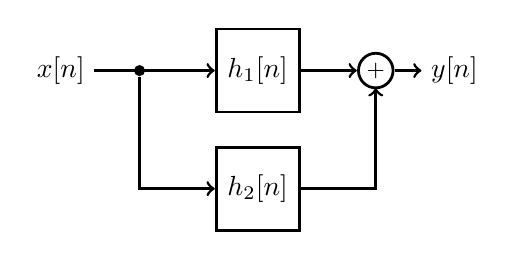
\begin{tikzpicture}
    \tikzstyle{block} = [draw, shape=rectangle, minimum height=3em, minimum width=3em, node distance=1.5cm, line width=1pt]
    \tikzstyle{sum} = [draw, shape=circle, node distance=1.5cm, line width=1pt, minimum width=1.25em]
    \tikzstyle{branch} = [fill,shape=circle,minimum size=4pt,inner sep=0pt]
    
    \node [left] at (0,0) (in) {$x[n]$};
    \node [branch, right of = in] (b1) {};
    \node [block, right of = b1] (h1) {$h_1[n]$};
    \node [block, below of = h1] (h2) {$h_2[n]$};
    \node [sum, right of = h1] (sum) {};
    \node at (sum) (plus) {\footnotesize$+$};
    \node [right of = plus] (out) {$y[n]$};
    
    \begin{scope}[line width=1pt]
    \draw [->] (in) -- (h1);
    \draw [->] (b1) |- (h2);
    \draw [->] (h2) -| (plus);
    \draw [->] (h1) -- (plus);
    \draw [->] (plus) -- (out);
    \end{scope}
\end{tikzpicture}
\vspace{1.5cm}

\plotsequence{{0/-1, 2/0, 0/1, 0/2, 0/3}}{$h_p[n]$}

\end{minipage}

Die Impulsantworten addieren sich. In diesem Fall werden die beiden IIR-Systeme zu einem FIR-System, da sich die Impulsantworten so überlagern, dass sich die unendlichen Reihen subtrahieren (Gut erkennbar mit Abbildung \ref{fig:g2} und \ref{fig:h2}, da $g_2[n] = h_1[n]$).